\documentclass{article}
\usepackage{fullpage}
\usepackage{amsfonts}
\usepackage{indentfirst}
\usepackage{enumerate}
\usepackage{graphicx}

\usepackage{titlesec}

\setcounter{secnumdepth}{4}

\titleformat{\paragraph}
{\normalfont\normalsize\bfseries}{\theparagraph}{1em}{}
\titlespacing*{\paragraph}
{0pt}{3.25ex plus 1ex minus .2ex}{1.5ex plus .2ex}

\title{\textbf{Notes for Semppr NSE - Exchange}}

\author{Preston Hewgley}

\begin{document}
\maketitle

\section{March 12: Comparing MCMC and Evolution simulation for generation of auxiliary variables}

\subsection{Eta Distributions}

\subsubsection{Phi=0}
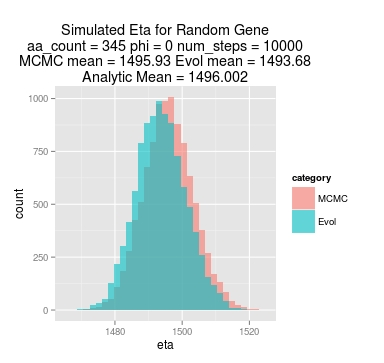
\includegraphics[scale=.65]{../eta_distbns/0_phi.jpg}
\subsubsection{Phi=0.01}
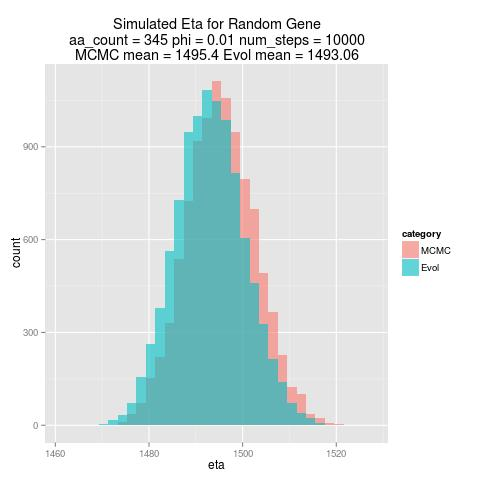
\includegraphics[scale=.5]{../eta_distbns/001_phi.jpg}
\subsubsection{Phi=0.1}

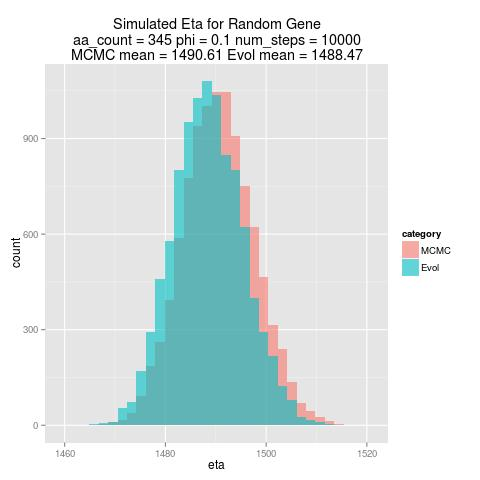
\includegraphics[scale=.5]{../eta_distbns/01_phi.jpg}
\subsubsection{Phi=1}
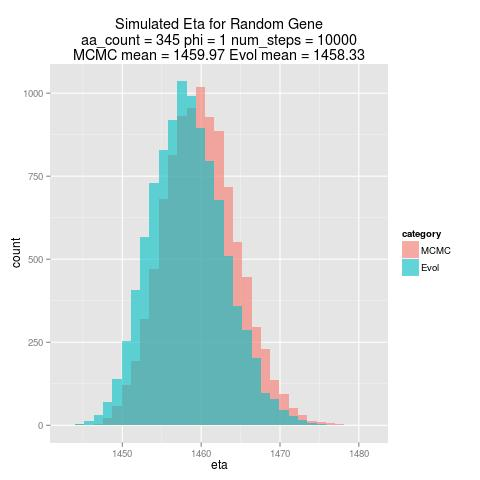
\includegraphics[scale=0.5]{../eta_distbns/1_phi.jpg}
\subsubsection{Phi=10}
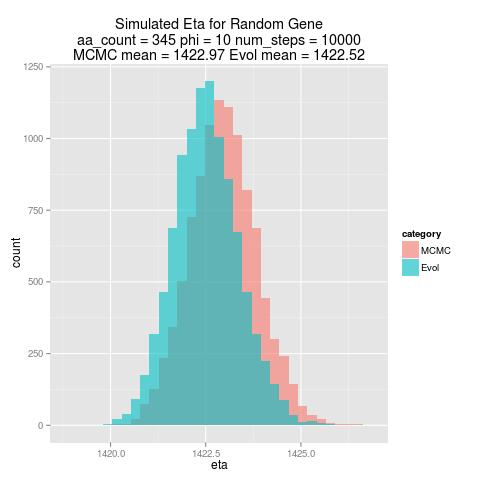
\includegraphics[scale=0.5]{../eta_distbns/10_phi.jpg}

\subsection{Runtime}
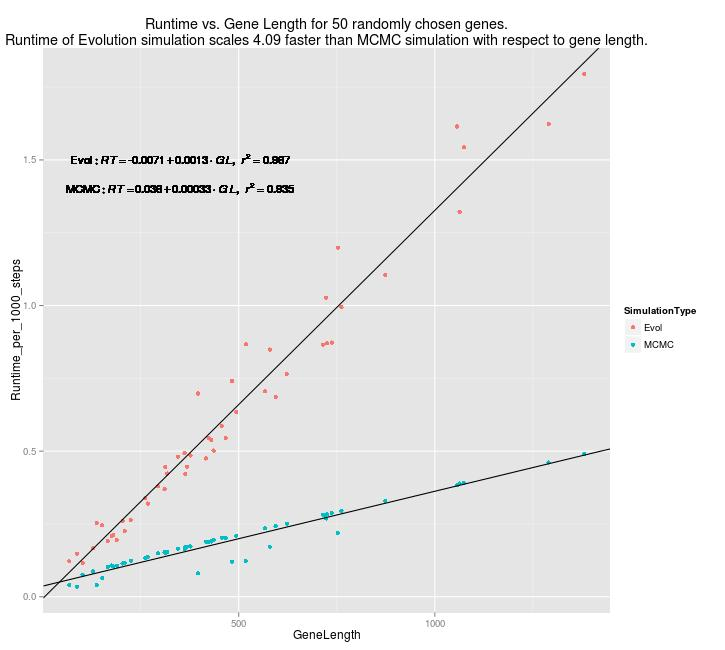
\includegraphics[scale=0.5]{../runtime/Runtime_plot_random_50.jpg}
\subsection{Phi Prediction}
\subsubsection{Evolution Simulation}
\includegraphics[scale=0.5]{../random_50/EVOL/250_steps/BIS5GMT-5/Rough_plot.jpeg}
\subsubsection{MCMC}
\includegraphics[scale=0.5]{../random_50/MCMC/250_steps/BIS10/Rough_plot.jpeg}
\newpage
\section{April 2: Verifying Phi Prediction using MCMC for Aux Vars}
\subsection{Profile MCMC Code}

I could not find an easy way to profile C code called from R and wanted to spend time on other tasks, so I'm still working on this.

\subsection{Check consistency between $\pi$ and likelihood calculations}
Last week we thought that an inconsistency concerning the haploid/diploid models for fixation probability $\pi$ and likelihood might be causing the slight discrepancy in the eta distributions generated by the evolution and MCMC codon sequence simulations.
From Sella and Hirsh (2005), for a Wright-Fisher process, the probability of fixation $\pi$ equals:
\begin{equation}
\pi(i->j) = \displaystyle{\frac{1-\left(\frac{f_i}{f_j}\right)^a}{1-\left(\frac{f_i}{f_j}\right)^{2N_e}}}
\end{equation}
where $a=1$ for diploid and $a=2$ for haploid. Also, 
\begin{equation}
Lik(\vec{c}|\vec{\lambda}) = \frac{(f_i)^\nu}{\sum_K(f_k)^\nu}
\end{equation}
where $\nu = 2Ne-1$ for diploid and $\nu = 2(Ne-1)$ for haploid. I verified both the MCMC and Evolution simulation code used the Wright-Fisher process diploid model.

\subsection{New Dataset}

 I took a new dataset out of the S. cerevisiae genome consisting of four genes from every fourth percentile of phi. Within every fourth phi percentile, I took one gene from each length quanitle.\\
 \\
 Ex. 1) Find genes within 0-4th phi percentile \\
 2) Store genes at 0, 25, 50, and 75 percentile length within this subset\\
 3) Find genes within 4-8th phi percentile\\
 4) Store genes at 0, 25, 50, and 75 percentile length within this subset\\
 
 Phi is rescaled so that median = 1.
 \pagebreak
 \subsection{Increase # phi steps}
	
	 \subsubsection{1000 Phi Steps}
	 
	 	\paragraph{Non-log scale}	 	
	 	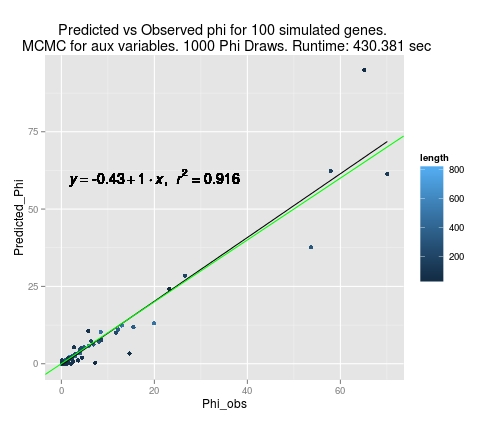
\includegraphics[scale=0.5]{../chosen_100/1000_steps/BIS10/Rplot01.jpeg}
	 	\paragraph{Log Scale}\\
	 	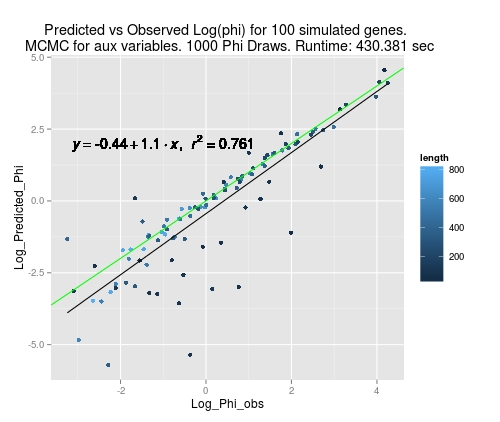
\includegraphics[scale=0.5]{../chosen_100/1000_steps/BIS10/Rplot02.jpeg}
	 	
	 \subsubsection{3000 Phi Steps}
	 
	 	\paragraph{Non-log scale}
	 	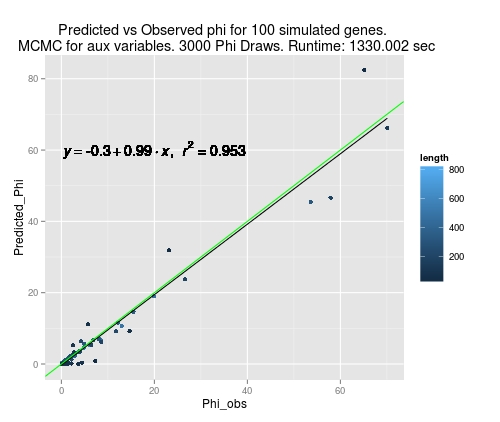
\includegraphics[scale=0.5]{../chosen_100/3000_steps/BIS10/Rplot01.jpeg}
	 	\paragraph{Log Scale}
		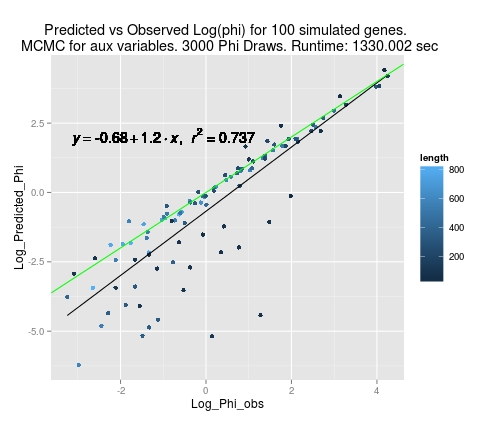
\includegraphics[scale=0.5]{../chosen_100/3000_steps/BIS10/Rplot02.jpeg}	 
 
 \subsection{Look @ Autocorrelation}

	Upon Wei-Chen's advice, I used the pacf {stats} function to look at the partial auto-correlation for each phi time-series. Wei-Chen advised the use of partial auto-correlation for MCMC because MCMC draws are naturally highly auto-correlated. Below are examples of some of the pacf plots, starting with the most highly auto-correlated and ending with the least. Based on these plots, Wei-Chen recommended that we thin our samples every 5 or 10 samples. 
	
	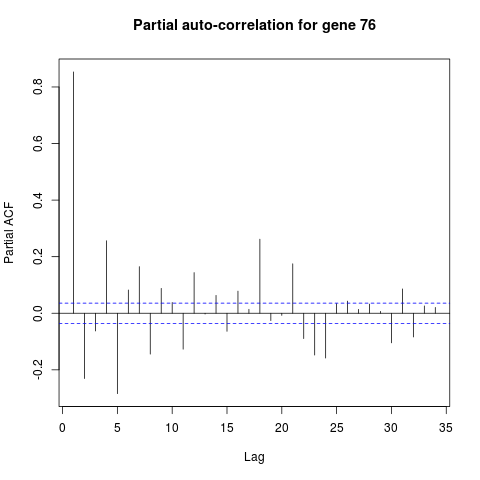
\includegraphics[scale=0.5]{../chosen_100/3000_steps/BIS10/pacf/76_pacf.png}
	
	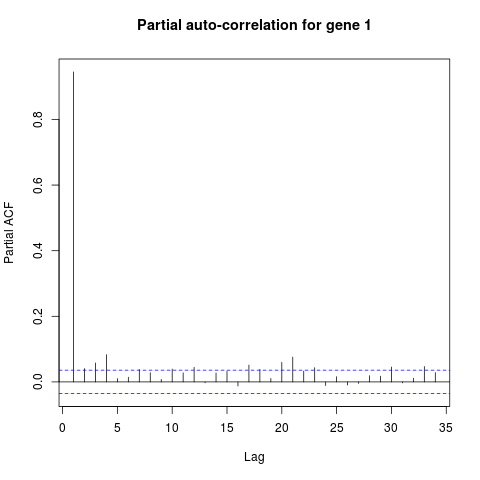
\includegraphics[scale=0.5]{../chosen_100/3000_steps/BIS10/pacf/1_pacf.png}
	
	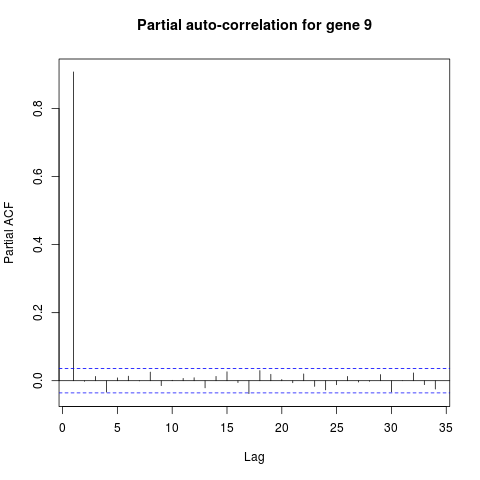
\includegraphics[scale=0.5]{../chosen_100/3000_steps/BIS10/pacf/9_pacf.png}
 
 \subsection{Plot Posterior Samples}
 
 
\section{April 9: Further verify Phi Prediction}
 	\subsection{Notes from April 2 Meeting}
	\begin{itemize}
 		\item Posterior Samples - Plot histogram and traces side by side with analytic $\bar\eta$, $\sigma^2_\eta$, and $\eta_{obs}$?
 		\item Make $\phi$ proposal adapt its variance to a target acceptance ratio
 		\item Start sequence MCMC at random sequence
 		\item Reflecting normal distribution for $\phi$ proposal? - asymmetric proposal distribution, need to account for this in acceptance ratio. ** Not asymmetric: q'/q=1 
	\end{itemize}

	\subsection{Objectives}
	\begin{itemize}
	\item Change dataset to include one gene from each phi percentile with random length - Complete
	\item Allow $\phi$ proposal variance to adapt to a target acceptance rate - Complete
	\item Provide option for a reflecting normal $\phi$ proposal - Complete
	\item Start aux variable simulation from random codon sequence to ensure the process is independent from previous samples - Complete
	\item Plot posterior samples and traces side by side
	\end{itemize}
 	\subsection{New New Test Dataset}
 	The new test dataset consists of one randomly chosen gene from every $\phi$ percentile of the S. cerevisiae genome. Genes were filtered by length so that only genes with length between 200 and 1000 were chosen. The new dataset can be found in ces3/branches/exchange/data/Rdata/chosen.100.philength.percentiles.dat
 	\subsection{Phi Prediction}
 	 
 	
	\subsubsection{Lognormal Phi Proposal} 	
 	 	
 	Below are the predicted phi values plotted against observed phi values for 100 simulated genes. Lognormal phi proposal adapts to an acceptance rate of 35-40\% as suggested by Gelman. Predicted phi was calculated from 300 posterior sample draws. 3000 samples were initially taken, and the first 1500 were discarded. The remainder was thinned by taking every fifth sample. 
 	
 	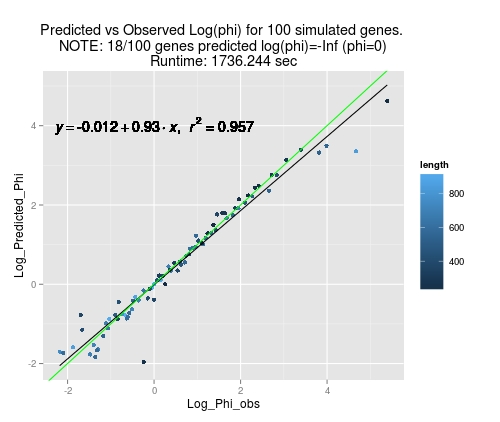
\includegraphics[scale=0.5]{../chosen_100/3000_steps/BIS10/lnorm_prop/Rplot.jpeg}
 	
	 Instead of helping genes recover from low phi levels, it made 18/100 genes "bottom out" at $log(\phi)=-\infty$ after going below the limits of numerical precision. 
	 
	 I also noticed that the model does not accurately predict phi for extremely high expression genes. The $\eta_{obs}$ in these genes is very close to the $\eta_{min}$, and I believe the discreteness of the states in this case plays a large role in the difficulty of predicting phi.
 	
 	Here are some examples of traces that bottomed out at phi=0. Traces consist of all 3000 samples.
 	
 	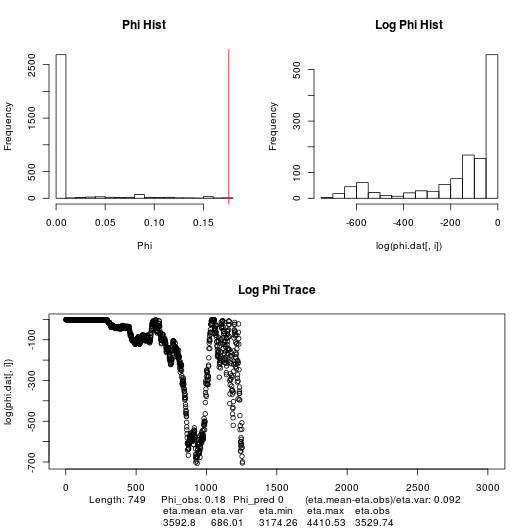
\includegraphics[scale=0.5]{../chosen_100/3000_steps/BIS10/lnorm_prop/hist/11_phi_hist.png}
 	
 	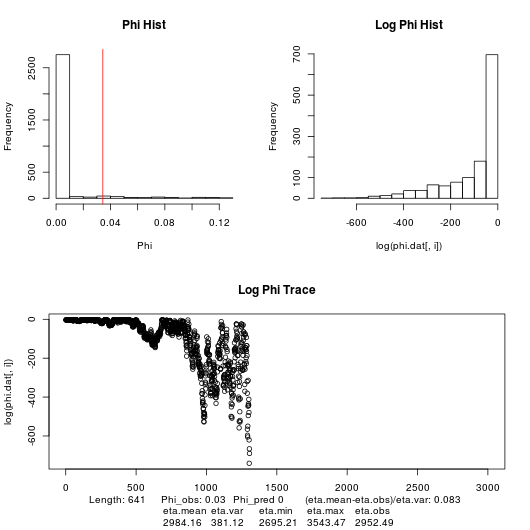
\includegraphics[scale=0.5]{../chosen_100/3000_steps/BIS10/lnorm_prop/hist/21_phi_hist.png}
 	
 	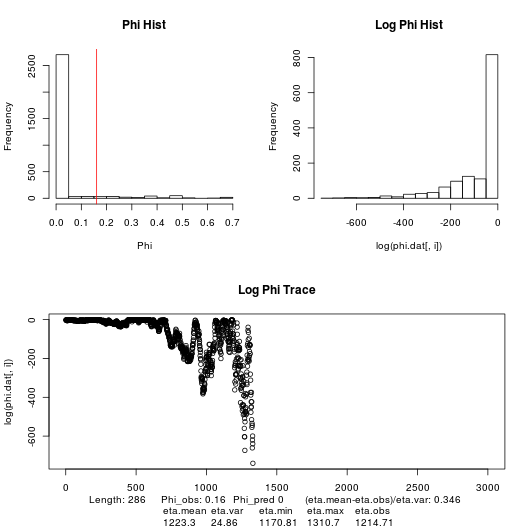
\includegraphics[scale=0.5]{../chosen_100/3000_steps/BIS10/lnorm_prop/hist/83_phi_hist.png}
 	
 	\pagebreak
 	Here are some examples of phi traces of very high expression genes. Traces consist of all 3000 samples. As you can see, the observed $\eta$ is very close to $\eta_{min}$ in these cases.
 	
 	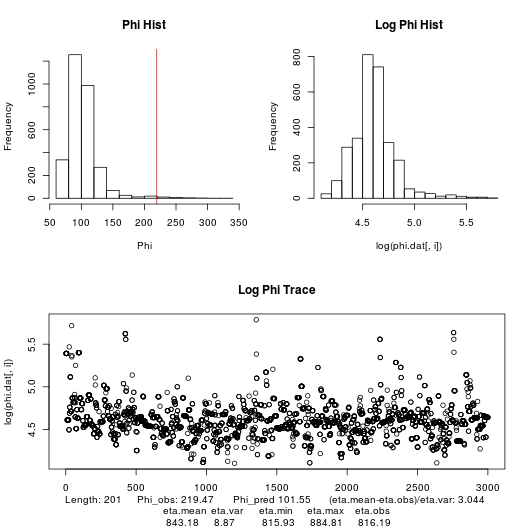
\includegraphics[scale=0.5]{../chosen_100/3000_steps/BIS10/lnorm_prop/hist/100_phi_hist.png}
 	
 	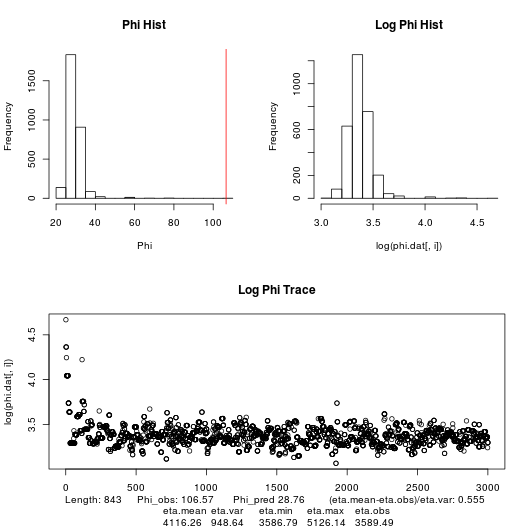
\includegraphics[scale=0.5]{../chosen_100/3000_steps/BIS10/lnorm_prop/hist/8_phi_hist.png}
 	
 	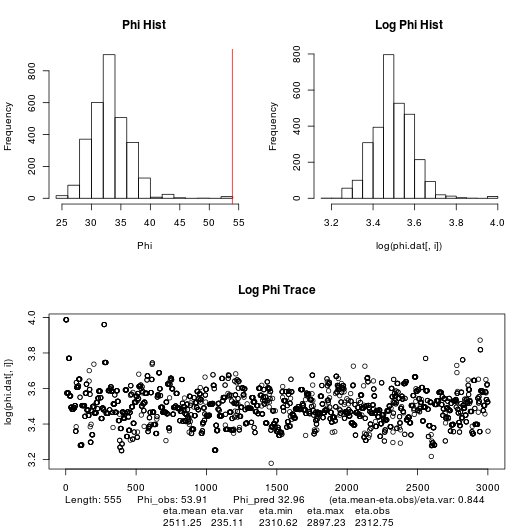
\includegraphics[scale=0.5]{../chosen_100/3000_steps/BIS10/lnorm_prop/hist/43_phi_hist.png}
 	 	
 	\subsubsection{Reflecting Normal Phi proposal}
 	
 	The Reflecting normal phi proposal resulted in better phi prediction. Below are the predicted phi values plotted against observed phi values for 100 simulated genes. Reflecting normal phi proposal adapts to an acceptance rate of 35-40\% as suggested by Gelman). Predicted phi was calculated from 300 posterior sample draws. 3000 samples were initially taken, and the first 1500 were discarded. The remainder was thinned by taking every fifth sample. None of the genes bottomed out at phi=0.
 	
 	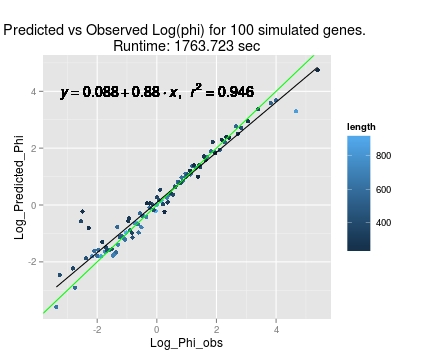
\includegraphics[scale=0.5]{../chosen_100/3000_steps/BIS10/reflnorm_prop/norand/Rplot01.jpeg}
 	
	\pagebreak 	
 	
 	Here are the traces of the same genes shown for the lognormal proposal. These genes have low expression.
 	
 	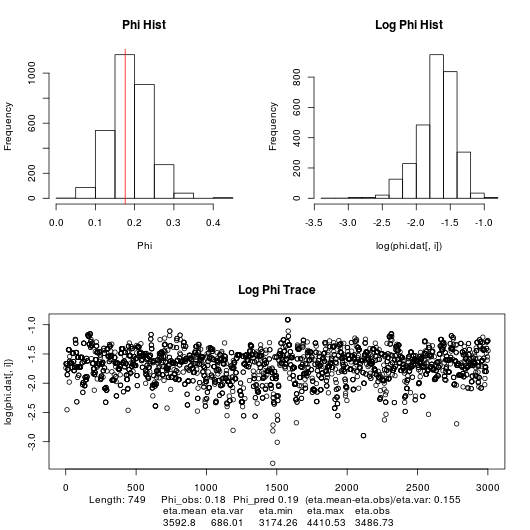
\includegraphics[scale=0.5]{../chosen_100/3000_steps/BIS10/reflnorm_prop/hist/11_phi_hist.png}
 	
 	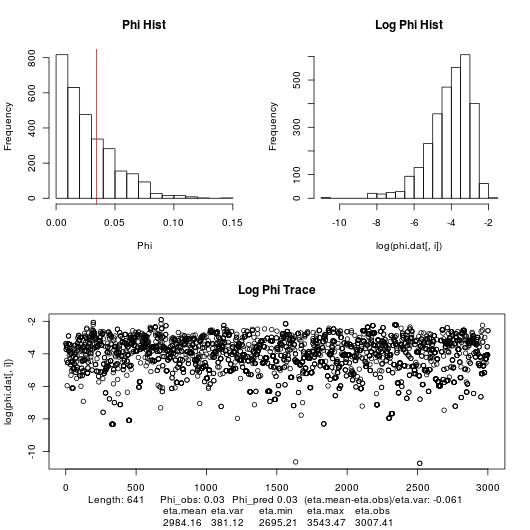
\includegraphics[scale=0.5]{../chosen_100/3000_steps/BIS10/reflnorm_prop/hist/21_phi_hist.png}
 	
 	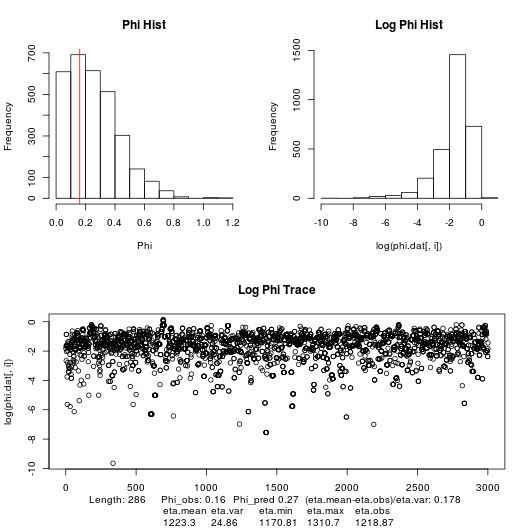
\includegraphics[scale=0.5]{../chosen_100/3000_steps/BIS10/reflnorm_prop/hist/83_phi_hist.png}
 	
 	
	These genes have very high expression.
 	
 	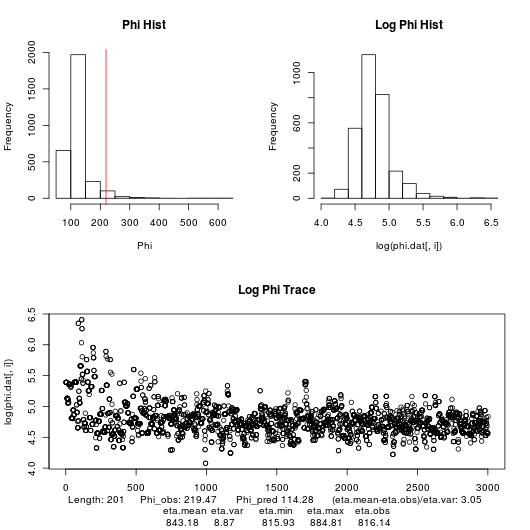
\includegraphics[scale=0.5]{../chosen_100/3000_steps/BIS10/reflnorm_prop/hist/100_phi_hist.png}
 	
 	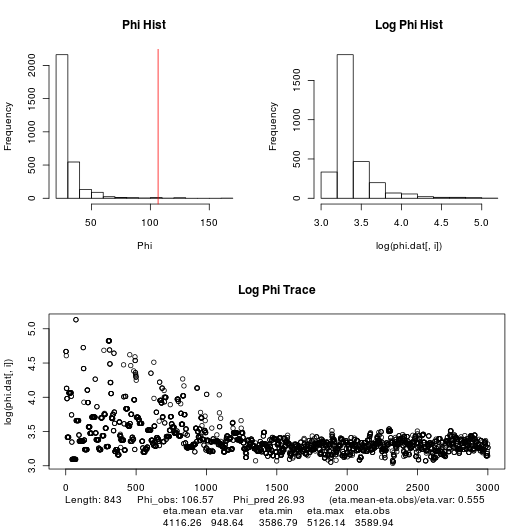
\includegraphics[scale=0.5]{../chosen_100/3000_steps/BIS10/reflnorm_prop/hist/8_phi_hist.png}
 	
 	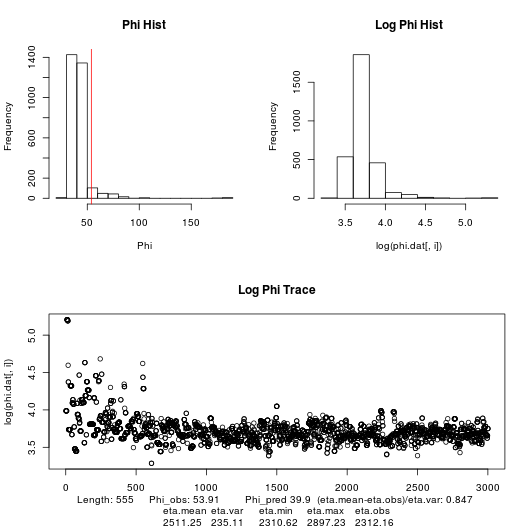
\includegraphics[scale=0.5]{../chosen_100/3000_steps/BIS10/reflnorm_prop/hist/43_phi_hist.png}
 	
 	\subsection{Under-predicting High Expression Genes}
	 	
	 	We noticed that the model was under-predicting phi for high-expression genes. My first thought was that the simulated genes may not have been burned in for long enough to reach stationarity. After increasing the amount of time the simulated genes were burned in, the phi prediction on these genes was much more accurate. This indicates that the problem was not in the model but the simulated data. Below is the corresponding plot of log predicted phi vs. log real phi. Both the slope and $R^2$ are very close to one, which is what we would expect for perfect prediction. 
	 	
	 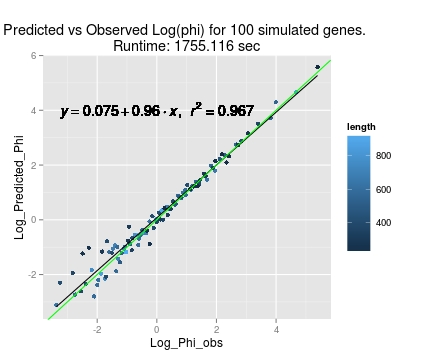
\includegraphics[scale=0.5]{../chosen_100/3000_steps/BIS10/reflnorm_prop/norand/Rplot.jpeg}
 		
 	\subsection{Conclusion}
 	
	 	The adaptive reflecting normal phi proposal produces the best phi predictions.
 	
 	\subsection{Next Steps}
 		\begin{enumerate}
 		\item Currently, the model starts phi at the observed value. The next step should start phi from a random value to verify that phi burns in to the correct value.
 		\item Once we have verified that phi burns in to the correct value, we should test the model on real genome data.
 		\end{enumerate}
 
 \newpage
 
 \section{April 16: Phi burn-in and code profile}
 
	 \subsection{Phi burn-in}
	 
		As the final verification that phi prediction is working, phi was predicted on a simulated dataset starting from an initial phi value not equal to the correct value. If phi prediction is working, phi should burn in to the correct value, and we should see similar results to when phi began at the observed value. 

		All sequences were simulated under phi observed. All phi MCMC's started at phi=1. The MCMC ran for 3000 steps, the first 1500 were discarded, and the remaining 1500 were thinned by taking every fifth sample. This phi prediction produced similar results to when phi began at phi observed, which suggests that our phi prediction is working as we expected.
		
		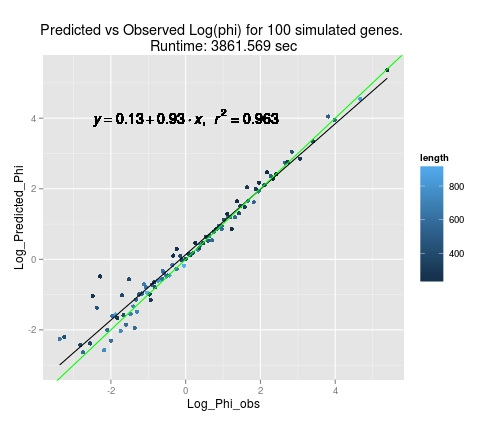
\includegraphics[scale=0.5]{../chosen_100/3000_steps/BIS10/reflnorm_prop/phistart-1/Rplot.jpeg}
		
		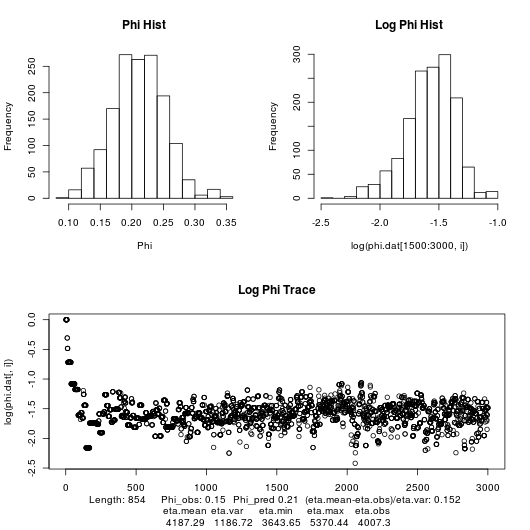
\includegraphics[scale=0.5]{../chosen_100/3000_steps/BIS10/reflnorm_prop/phistart-1/hist/7_phi_hist.png}
		
 		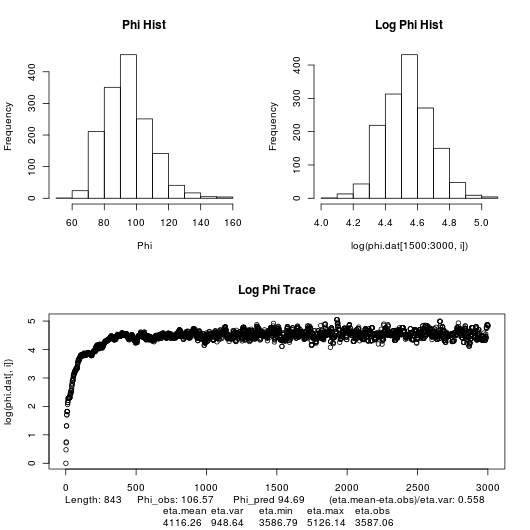
\includegraphics[scale=0.5]{../chosen_100/3000_steps/BIS10/reflnorm_prop/phistart-1/hist/8_phi_hist.png}
 		
		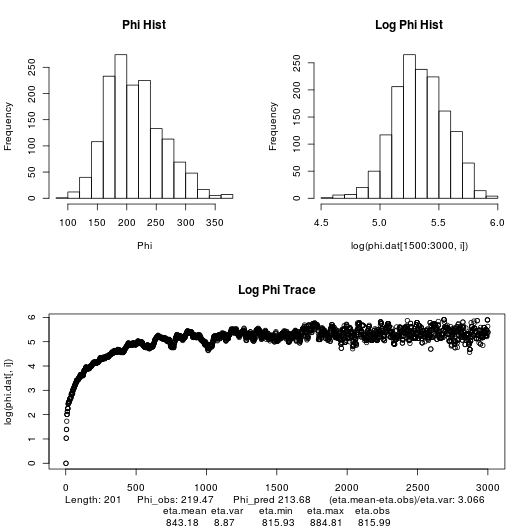
\includegraphics[scale=0.5]{../chosen_100/3000_steps/BIS10/reflnorm_prop/phistart-1/hist/100_phi_hist.png}

\newpage	 	
	 	
	 \subsection{Profile}
	 
	 I found a program to profile the C code, but it's not giving me much useful information right now. I'm still trying to find a better way to profile.
	 
	 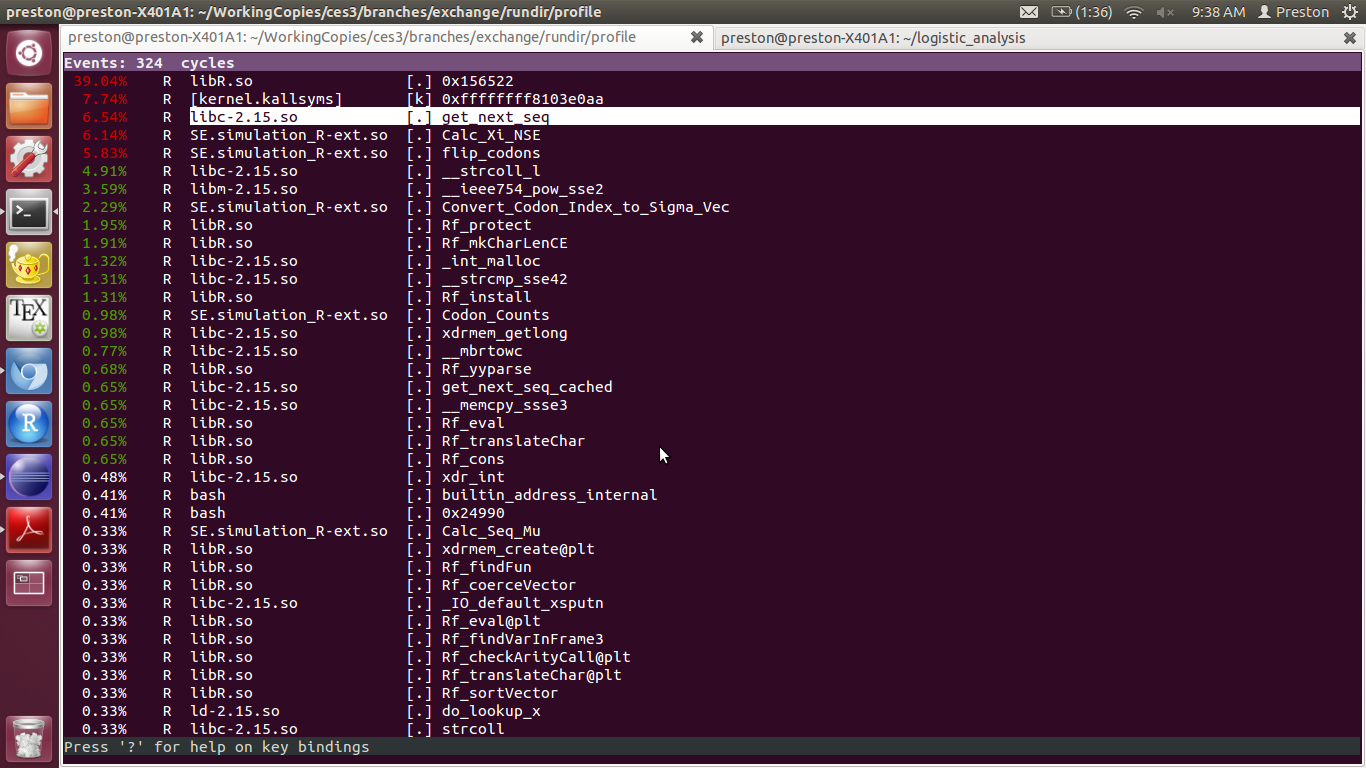
\includegraphics[scale=0.4]{../profile/profile.png}
	 
 \section{April 24: Profile, Stationarity, SCUO, Larger Dataset}
 
 \subsection{Profile}
 
 	A profile of the code revealed some bottlenecks. Optimizing the code at these bottlenecks sped up the auxiliary variable generation by ~3x. Below are timing tests before and after optimization.
 	
 	\subsubsection{Before Optimization}
 	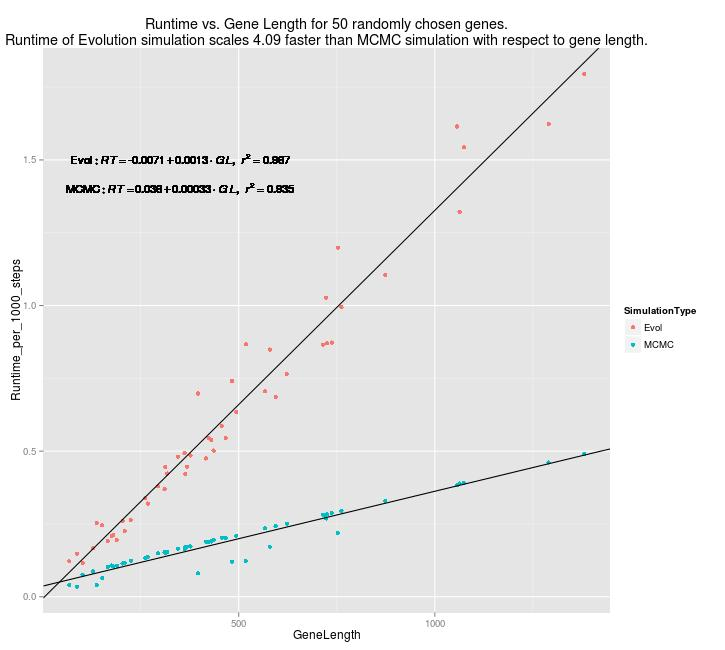
\includegraphics[scale=0.5]{../runtime/Runtime_plot_random_50.jpg}
 	
 	\subsubsection{After Optimization}
 	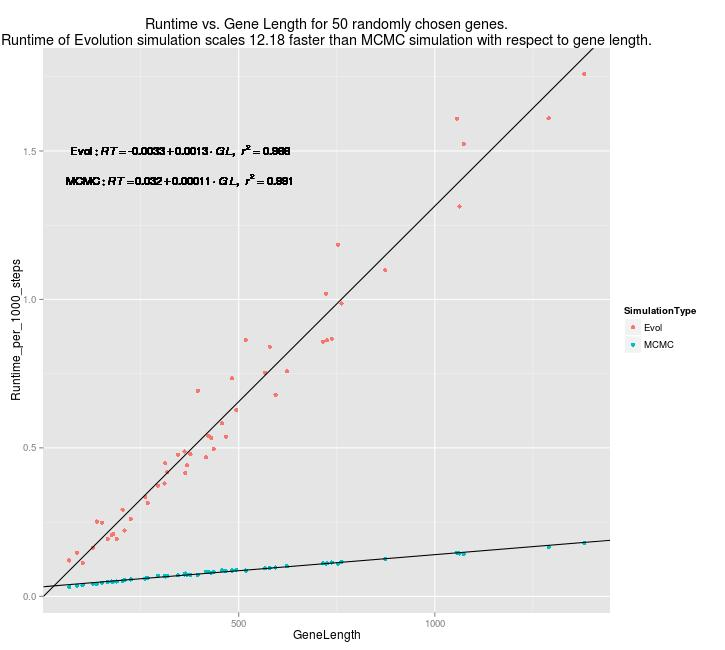
\includegraphics[scale=0.5]{../runtime/Runtime_plot_random_50_after_profile.jpg}
 \newpage
 \section{May 1: Stationarity, SCUO, Larger Dataset (cont'd)} 	
 	
 \subsection{SCUO}
 	
 	SCUO now gives us a reference to guess an initial phi based on a lognormal distribution with mean 0. This method is the same method Wei-Chen has been using.
 	
 \subsection{Stationarity}
 
 	Stationarity is assessed based on a modified Gelman convergence criteria. In the normal criteria, several chains start at random points in parameter space and run until the chains converge. Starting multiple chains would be too computationally intensive, so one chain is divided into 10 different chains that are treated as independent chains. This method could indicate convergence prematurely, but we can adjust the convergence threshold to compensate if necessary.
 	
 \subsection{Larger Dataset}

	\subsubsection{Phi prediction and runtime}
	
	Phi prediction on a set of 1000 simulated genes showed high accuracy. Initial phi was guessed based on SCUO and phi draws were taken for a gene until that gene's phi trace reached stationarity.  The phi prediction lasted 2944.09 seconds, which is significantly faster than the performance before optimizing the code. Before, phi prediction on 100 genes took 3861.57 sec.
 
 	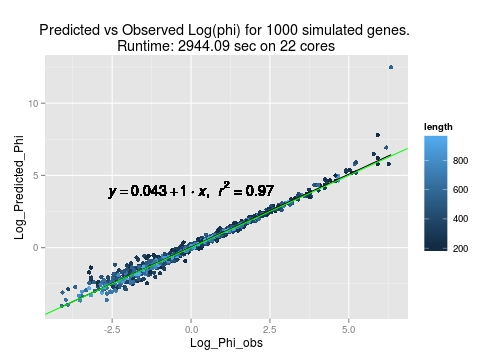
\includegraphics[scale=0.5]{../1000_test/scuo_conv/Rplot.jpeg}
 	
 	\subsubsection{Stationarity}
 	
 	The minimum allowed phi steps was 500 and the maximum was 3000. 998 genes reached stationarity before the maximum. One of the genes that did not reach stationarity was the gene with highest expression and the other gene was a pretty average gene. The gene with highest expression did not reach stationarity because the simulated sequence was the optimal sequence. In this case, the algorithm will only accept if $\phi_{prop} > \phi_{curr}$. This case should never pose a problem with real data since observing an optimal sequence is very unlikely. I'm still not sure why the other gene did not reach stationarity. The phi trace appeared to converge, but apparently the chain did not reach the convergence threshold. The below plot shows the trace. 
 	
 	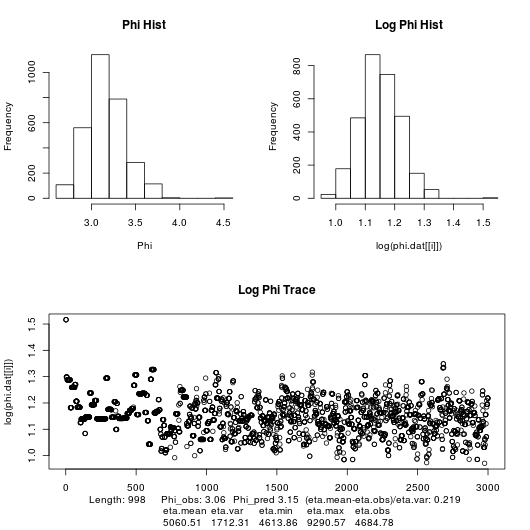
\includegraphics[scale=0.5]{../1000_test/scuo_conv/hist/999_phi_hist.png}
\newpage
 \section{May 15: Estimating Elongation Rate Parameter}

	\subsection{Elong Rate Estimation w/ $\phi$}
 
 	An additional step in the outer MCMC can pull draws from the posterior distribution of genome-wide parameters. By generating an aux. variable from each gene in the genome, we can calculate a combined acceptance ratio for all genes at once. 
	\begin{equation}
	a = \displaystyle{\prod_{i=1}^{\#\,genes}\frac{f(\vec{c}_{obs,i}|\phi,\vec{\lambda}^\prime)p(\vec{\lambda}^\prime)q(\vec{\lambda}|\vec{\lambda}^\prime,\phi)}{f(\vec{c}_{obs,i}|\phi,\vec{\lambda})p(\vec{\lambda})q(\vec{\lambda}^\prime|\vec{\lambda},\phi}\frac{f(\vec{c}_{sim,i}|\phi,\vec{\lambda})}{f(\vec{c}_{sim,i}|\phi,\vec{\lambda}^\prime)}}
	\end{equation}	 	
	
 	As a test, this combined acceptance ratio was used in an MCMC to estimate one elongation rate in a 2-codon amino acid with known phi. The MCMC used a simulated dataset of 100 genes and held phi constant at its true value. Elong rate MCMC was started at its true value and new elong rates were proposed with random walk lognormal distribution with variance 0.5, resulting in 14.2\% acceptance rate. Runtime lasted 1488.1 sec for 1000 steps. This method takes significantly longer per gene than estimating phi only because each step requires all genes. Therefore, genes cannot be removed after reaching stationarity. Below shows the trace and histogram of the elong rates. As the plot shows, the trace converges near the correct value.
 	
 	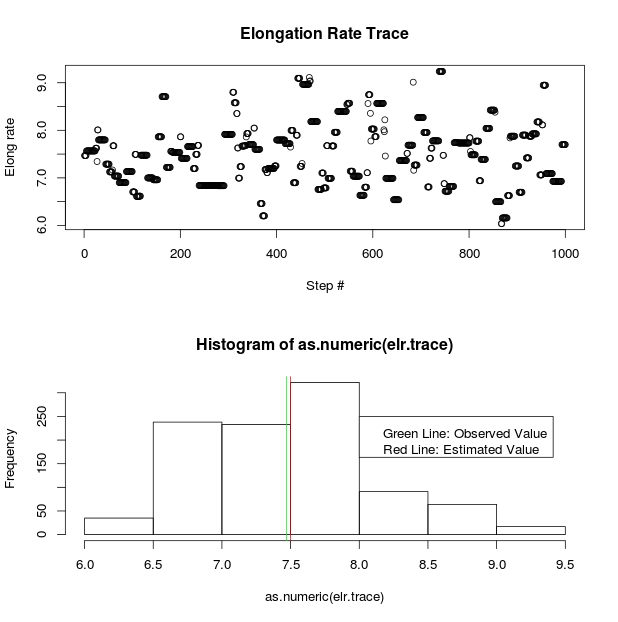
\includegraphics[scale=0.5]{../chosen_100/genome_parms/elr_test/Rplot.jpeg}
 	
	\subsection{Elong Rate Estimation w/o $\phi$} 	 	
 	
 	The next test verifies that phi and elong rate can be estimated simultaneously. This test estimated elong rate as in the previous example without knowing phi. Elong rate is proposed based on a random walk lognormal distribution with variance 0.1, resulting in a 55.4\% acceptance rate. Phi is guessed based on SCUO. The plots below show the trace and histogram of estimated elong rate along with a plot of predicted vs obs phi.
 	
 	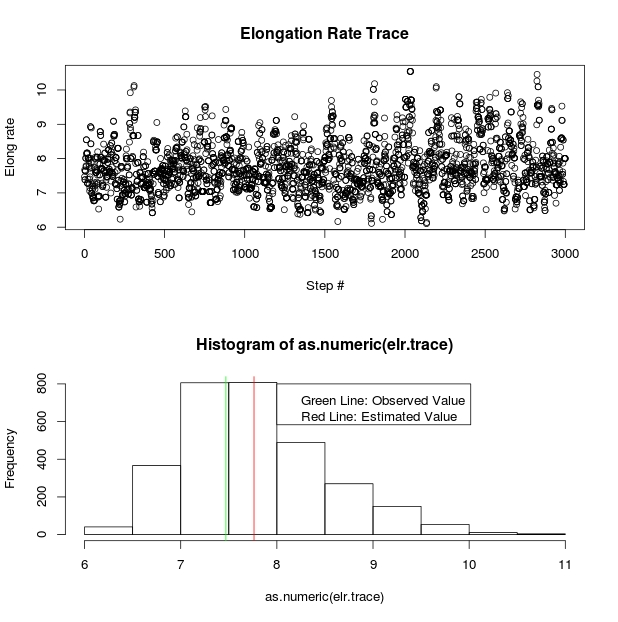
\includegraphics[scale=0.4]{../chosen_100/genome_parms/elr_test_wo_phi/Rplot.jpeg}
 	
 	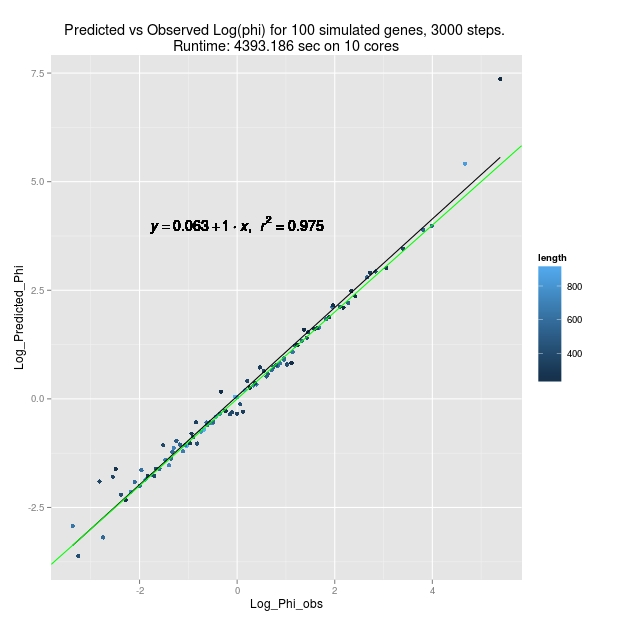
\includegraphics[scale=0.4]{../chosen_100/genome_parms/elr_test_wo_phi/Rplot01.jpeg}
	
	\subsection{Elong Rate Burn-in}	
	 	
 	Another test verifies that elong rate can burn in correctly. This test is essentially the same as the last one, but elong rate is started at an arbitrary value away from the observed value
 	
	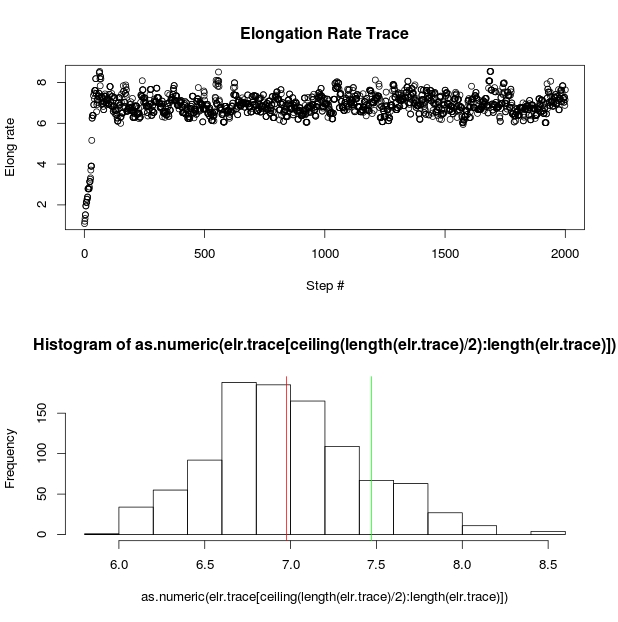
\includegraphics[scale=0.4]{../chosen_100/genome_parms/elr_test_wo_phi_init_elr/Rplot.jpeg}
 	
 	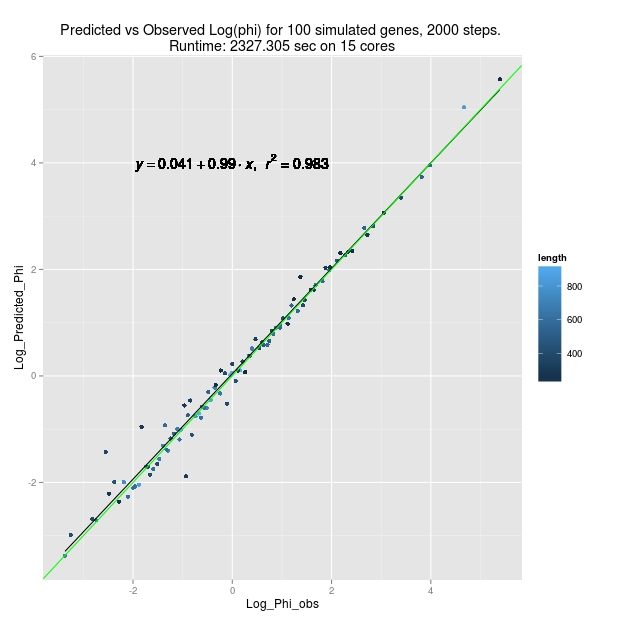
\includegraphics[scale=0.4]{../chosen_100/genome_parms/elr_test_wo_phi_init_elr/Rplot01.jpeg}
 	
 	\subsection{Next Steps}
 	
 	\begin{enumerate}
 		\item Prior for elong rate??
 		\item Modify MCMC to predict mutation rate and elongation rate of a 2-codon AA based on a multivariate normal distribution
 		\begin{itemize}
 			\item Generate covariance matrix
 			\item Make covariance matrix adapt to acceptance rate of 25-35%
 		\end{itemize}
 		\item Extend MCMC to predict mutation rate and elongation rate for all codons
 	\end{enumerate}
\newpage
	\subsection{Notes on next steps}
	
	\subsubsection{Multivariate Normal}
	
	Mutation and elongation rates should be proposed from a multivariate normal distribution with mean array $\mu$ and covariance matrix $\Sigma$, where
	\begin{equation}
		\mu = \[ \left( \begin{array}{c}
				\mu_{elr} \\
				\mu_{mut} \end{array} \right)\]
	\end{equation}
	\begin{equation}				
	    \Sigma = \[ \left( \begin{array}{cc}
		     		\sigma_{elr}^2 & \rho\sigma_{elr}\sigma_{mut} \\
			     	\rho\sigma_{elr}\sigma_{mut} & \sigma_{mut}^2 \end{array} \right)\]
	\end{equation}
	
	Question: What is correlation coefficient $\rho$ equal to? It would seem like $\rho=0$ since elongation rate and mutation rate are independent properties. This would also simplify the covariance matrix so we could essentially pull from two independent random normal distributions instead of one multivariate normal. 
 	
\end{document}